\section{Architettura di Rete}\label{architettura-di-rete}

La topologia e' suddivisa logicamente in due reti:

\begin{itemize}
\tightlist
\item
  \textbf{Una rete di produzione per ogni team}, dove la rete
  \(\text{production-}k\) identifica gli oggetti di rete usati per
  collegare i container vulnerabili alla rete per il team \(k\)
\item
  \textbf{Al piu' una rete di verifica per ogni team}, dove la rete
  \(\text{verify-}k\) identifica gli oggetti di rete ed i container
  duplicati utilizzati per la verifica richiesta dal \(\text{team-}k\)
\end{itemize}

Dunque lo schema di indirizzamento prevede una netta separazione tra lo
spazio di gioco del team \(k\), la rete WireGuard e la rete di Incus:

\begin{itemize}
\tightlist
\item
  \passthrough{\lstinline!10.k.0.0/24!}: e' la sottorete WireGuard per i
  membri del team \(k\).
\item
  \passthrough{\lstinline!10.k.1.0/24!}: e' la sottorete LAN per i
  container di produzione e per i cloni di verifica.
\item
  \passthrough{\lstinline!172.16.0.0/24!}: e' la sottorete gestita da
  \(\text{incusbr0}\) per fornire la connettività esterna e le reti OVN
  tramite NAT.
\end{itemize}

\subsection{\texorpdfstring{Rete
\(\text{production-}k\)}{Rete \textbackslash text\{production-\}k}}\label{rete-textproduction-k}

La rete \(\text{production-}k\) e' fatta cosi, contiene:

\begin{itemize}
\tightlist
\item
  \(\text{wg-}k\): dispositivo L3 gestito da WireGuard, fa da
  terminazione per il tunnel del team \(k\)-esimo. Ha come IP gateway:
  \passthrough{\lstinline!10.k.0.0/24!}
\item
  \(\text{br-team-}k\): dispositivo L2 gestito dal kernel Linux. Ha come
  IP gateway: \passthrough{\lstinline!10.k.1.0/24!}
\item
  \(\text{eth0}\): le interfacce di rete \(\text{eth0}\) dei container
  vengono collegate a \(\text{br-team-}k\).
\end{itemize}

\(\text{wg-}k\) serve per fronire ai membri del team \(k\) l'endpoint
per la connessione tramite VPN, in questo modo i membri del team saranno
connessi direttamente alla rete \(\text{production-}k\). Ogni membro ha
la sua configurazione WireGuard associata al suo peer impostato
sull'interfaccia \(\text{wg-}k\). Aggiungere un peer all'interfaccia
WireGuard significa permettere ad un client con una certa chiave
pubblica di collegarsi con un certo indirizzo ip (\textbf{cryptokey
routing}), dunque ogni membro del team \passthrough{\lstinline!k!} ha il
suo indirizzo nella sottorete \passthrough{\lstinline!10.k.0.0/24!}.

L'interfaccia \(\text{br-team-}k\) permette di creare una rete LAN per i
container del team \(k\). Ogni interfaccia
\passthrough{\lstinline!eth0!} dei container istanziati dal team \(k\),
vengono ``collegati'' (tramite l'utilizzo di un profilo Incus) a
\(\text{br-team-}k\). La connessione tra bridge e container viene
gestita direttamente da Incus.

Questo collegamento avviene tramite l'utilizzo di una
\passthrough{\lstinline!veth pair!} (Virtual Ethernet) per container:
una estremita e' collegata a \passthrough{\lstinline!br-team-k!},
l'altra all'interffacia del container \passthrough{\lstinline!eth0!}.
Dunque all'interno del kernel appesantiamo il carico nella gestione
delle interfacce, infatti avremmo oltre ad
\passthrough{\lstinline!eth0!}, una coppia
\passthrough{\lstinline!veth!} per ogni container.

\begin{quote}
\passthrough{\lstinline!veth!}: E' utile per collegare interfacce che
risiedono per esempio su differenti Network Namespace (ossia il modo in
cui sono implementati i container). Utilizzano poca CPU e poca memoria,
dato che l'implementazione risiede direttamente nel kernel. Dunque per
centinaia di \passthrough{\lstinline!veth!} non si ha un degrado
evidente delle prestazioni. \footnote{\label{fn:ref_15}https://dev.to/godofgeeks/virtual-ethernet-devices-veth-ofd}
\end{quote}

Tramite regole di routing, il traffico dell'interfaccia \(\text{wg-}k\)
viene instradato verso \(\text{br-team-}k\) e viceversa. Questa regola
viene applicata aggiungendo dentro al set
\passthrough{\lstinline!team\_links!} (una struttura dati all'interno
del kernel) la coppia di interfacce interessate.


\begin{figure}[htbp]
  \centering
  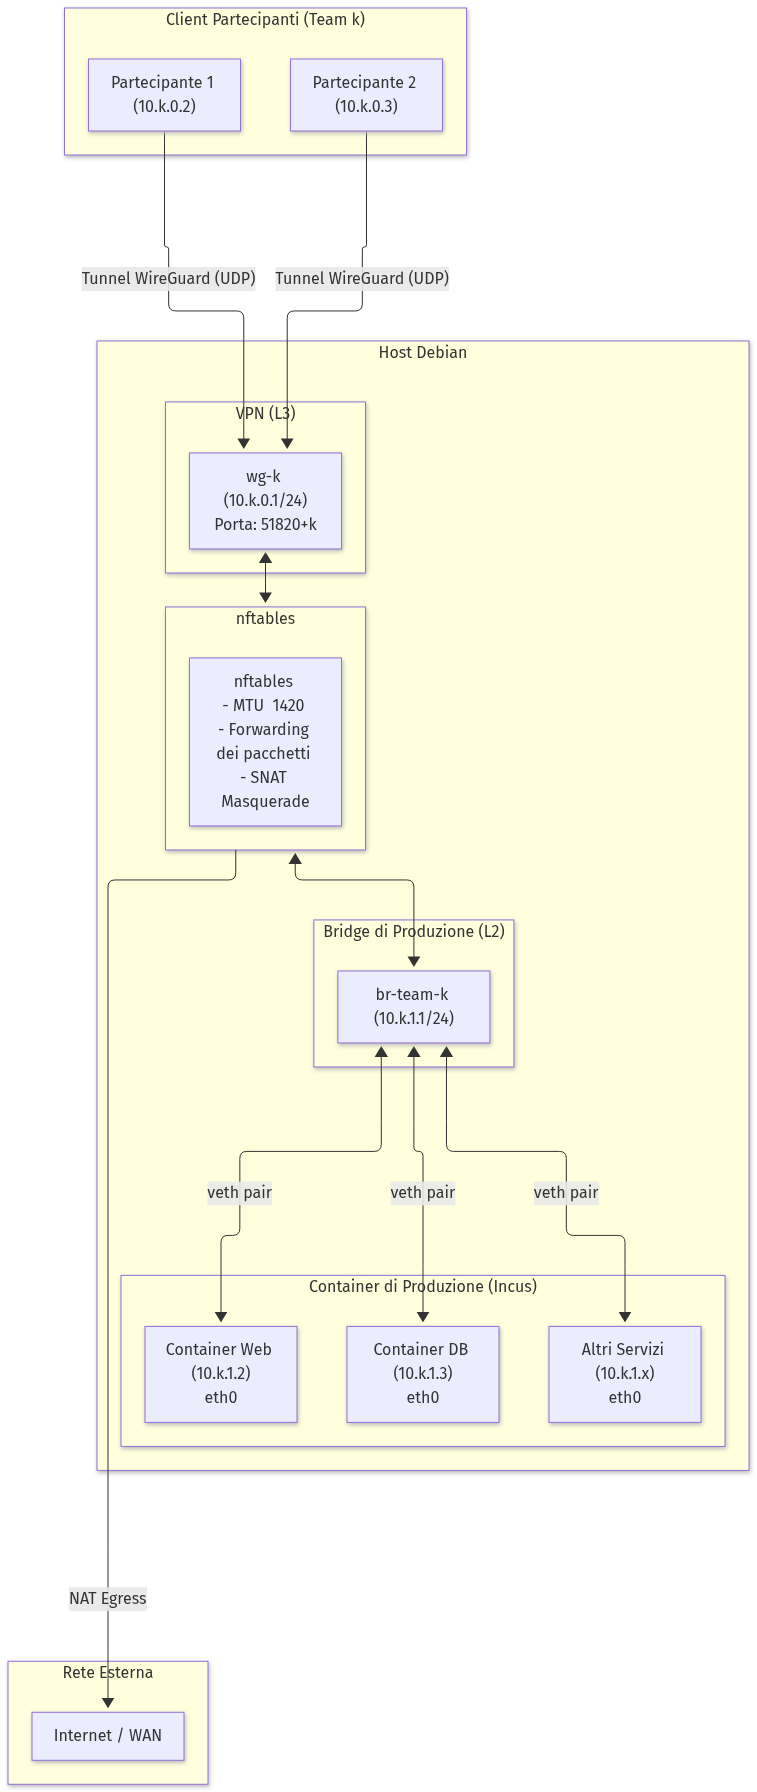
\includegraphics[width=0.92\linewidth,height=0.7\textheight,keepaspectratio]{src/images/mermaid_311_rete_production_k_fc40fab722.png}
  \caption{311 Rete Production K}
  \label{fig:mermaid_311_rete_production_k_fc40fab722}
\end{figure}


\begin{center}\rule{0.5\linewidth}{0.5pt}\end{center}

\subsection{\texorpdfstring{Rete
\(\text{verify-}k\)}{Rete \textbackslash text\{verify-\}k}}\label{rete-textverify-k}

La rete \(\text{verify-}k\) e' fatta cosi, contiene:

\begin{itemize}
\tightlist
\item
  \(\text{verify-ovn-}k\): rete virtuale logica gestita via SDN tramite
  OVN e orchestrata da Incus \footnote{\label{fn:ref_16}Documentazione ufficiale Incus,
    OVN network driver:
    https://linuxcontainers.org/incus/docs/main/reference/network\_ovn/}.
  Non costituisce una singola interfaccia di rete convenzionale del
  kernel, ma una topologia virtuale isolata composta da uno switch e un
  router con gateway: \passthrough{\lstinline!10.k.1.1/24!}.
\item
  \(\text{incusbr0}\): bridge di rete di Incus con gateway
  \passthrough{\lstinline!172.16.0.1/24!}. Svolge il ruolo di
  interfaccia per l'instradamento verso l'esterno della rete OVN.
\item
  \(\text{eth0}\): sono le interfacce di rete dei container clonati
  (\passthrough{\lstinline!10.k.1.x!}) che vengono collegate a
  \(\text{verify-ovn-}k\).
\end{itemize}

\begin{quote}
Incus e' in grado di gestire da solo il collegamento tra
\(\text{incusbr0}\) ed \(\text{verify-ovn-}k\). Questo semplifica di
molto la gestione delle interfacce di verifica per BlueAgent.
\end{quote}

Le interfacce dei container e la rete \(\text{verify-ovn-}k\) sono
gestite dalla SDN (\emph{Software Defined Network}).
\(\text{verify-ovn-}k\) e' implementata da:

\begin{enumerate}
\def\labelenumi{\arabic{enumi}.}
\tightlist
\item
  un \textbf{Logical Switch} (denominato internamente da Incus nel DB di
  OVN come \passthrough{\lstinline!incus-net<ID>-ls-int!} \footref{fn:ref_16}):
  rappresenta la LAN su cui si agganciano le interfacce virtuali dei
  container di verifica.
\item
  un \textbf{Logical Router} (denominato
  \passthrough{\lstinline!incus-net<ID>-lr!} \footref{fn:ref_16}):
  agisce come gateway (\passthrough{\lstinline!10.k.1.1/24!}),
  permettendo ai container clonati di preservare l'identica
  configurazione IP rispetto alla produzione.
\end{enumerate}

\begin{quote}
\textbf{Tunneling Geneve e considerazioni sull'MTU:} OVN impiega il
protocollo di tunneling \textbf{Geneve} (\emph{Generic Network
Virtualization Encapsulation}) \footnote{\label{fn:ref_17}Documentazione architetturale
  OVN e Geneve: https://docs.ovn.org/en/latest/topics/geneve.html} per
realizzare la rete overlay, incapsulando i frame L2 all'interno di
pacchetti UDP. Il tunnel Geneve opera interamente confinato all'interno
dell'host, isola il traffico di verifica impedendo che transiti sulle
interfacce di rete visibili ai partecipanti.
\end{quote}

L'incapsulamento Geneve introduce tuttavia un overhead di intestazione
di 58 byte, riducendo l'MTU effettiva della rete di verifica a \(1442\)
byte (rispetto ai 1500 byte standard). In combinazione con il tunnel
WireGuard (avente MTU \(1420\)), abbiamo una riduzione complessiva del
\emph{Path MTU}. Se pacchetti di dimensione eccedente hanno il flag
\emph{Don't Fragment} (DF) abilitato, rischiano di essere scartati
generando un fenomeno di \emph{Path MTU Blackhole}. Questo problema
viene risolto forzando il \emph{clamping} del MSS per il traffico TCP
via \passthrough{\lstinline!nftables!} \footnote{\label{fn:ref_18}Documentazione
  Netfilter, TCP MSS Clamping:
  https://wiki.nftables.org/wiki-nftables/index.php/Forwarding\_traffic},
mentre il traffico UDP deve rimanere entro i limiti imposti dall'MTU
minima della catena.

L'uso di una SDN garantisce l'assenza di conflitti di routing grazie a
una netta separazione tra \textbf{spazio utente} e \textbf{spazio
kernel} \footnote{\label{fn:ref_19}Documentazione Open vSwitch, architettura Datapath
  Kernel vs Userspace:
  https://docs.openvswitch.org/en/latest/intro/what-is-ovs/}:

\begin{itemize}
\tightlist
\item
  \textbf{Spazio Utente (Control Plane):} i demoni di controllo di OVN
  (\passthrough{\lstinline!ovn-controller!},
  \passthrough{\lstinline!ovn-northd!}) e di Open vSwitch
  (\passthrough{\lstinline!ovs-vswitchd!}) elaborano la topologia logica
  e la traducono in flussi OpenFlow. Il router OVN esiste puramente a
  livello logico.
\item
  \textbf{Spazio Kernel (Data Plane):} l'effettivo inoltro dei frame
  avviene ad alte prestazioni tramite il modulo kernel di Open vSwitch.
  Il kernel gestisce una tabella di flussi in cache (\emph{datapath flow
  cache}), instradando e modificando i pacchetti senza passare dallo
  stack di rete IP standard dell'host.
\end{itemize}

Il collegamento tra i container e la rete OVN sfrutta sempre una coppia
\passthrough{\lstinline!veth pair!}: un'estremità risiede all'interno
del container come \passthrough{\lstinline!eth0!}, mentre l'altra
estremità sull'host viene agganciata direttamente al bridge di Open
vSwitch.

\begin{quote}
\passthrough{\lstinline!SDN (Software Defined Networking)!}: Paradigma
architetturale che separa il \textbf{piano di controllo} dal
\textbf{piano dei dati}, consentendo di gestire e programmare
l'infrastruttura di rete interamente via software.

\passthrough{\lstinline!Open vSwitch (OVS)!}: Switch virtuale operante
nel kernel Linux come Data Plane. Sostituisce il classico bridge Linux
eseguendo l'inoltro dei frame ad alte prestazioni basandosi su tabelle
di flussi (\emph{flow tables}).

\passthrough{\lstinline!OpenFlow!}: Protocollo standard che permette al
controller SDN di comunicare con lo switch e programmare le regole di
matching e le azioni direttamente all'interno delle pipeline di Open
vSwitch.

\passthrough{\lstinline!OVN (Open Virtual Network)!}: Sistema SDN che
opera come Control Plane per Open vSwitch. Traduce topologie logiche
(Logical Switch, Logical Router, NAT e ACL) in flussi OpenFlow
distribuiti, istruendo Open vSwitch su come instradare il traffico senza
creare molteplici interfacce o bridge dedicati nel kernel host. E'
costituito da due interfacce: * \textbf{OVN Northbound}: e'
l'interfaccia dove dichiaro le reti che voglio creare e le loro
proprietà che devono rispettare. * \textbf{OVN Southbound (SB)
DB:}~Memorizza le tabelle di flussi logici compilate e le associazioni
di chassis (host fisici)
\end{quote}

La comunicazione verso l'esterno avviene collegando il Logical Router
OVN al bridge parent \(\text{incusbr0}\), da cui ottiene un indirizzo
IP. L'accesso a Internet sfrutta un meccanismo di NAT a due stadi:

\begin{itemize}
\tightlist
\item
  \textbf{SNAT in OVN}: quando un container
  (\passthrough{\lstinline!10.k.1.x!}) invia traffico all'esterno, il
  Logical Router riscrive l'indirizzo sorgente sostituendolo con l'IP
  uplink assegnato su \passthrough{\lstinline!incusbr0!}. Se non fosse
  applicato, i pacchetti in uscita manterrebbero l'indirizzo sorgente
  \passthrough{\lstinline!10.k.1.x!} e le risposte dall'esterno
  verrebbero erroneamente instradate verso l'ambiente di produzione.
\item
  \textbf{SNAT sull'host}: una volta raggiunto
  \passthrough{\lstinline!incusbr0!}, le regole
  \passthrough{\lstinline!nftables!} dell'host applicano la regola di
  masquerade verso l'interfaccia fisica per uscire su Internet.
\end{itemize}

Il NAT a due stadi e' necessario per evitare collisioni di routing
sull'host: il primo stadio ``nasconde'' gli indirizzi duplicati
\passthrough{\lstinline!10.k.1.x!} traducendoli in un IP univoco
sull'infrastruttura \passthrough{\lstinline!172.16.0.0/24!}, mentre il
secondo stadio permette la navigazione esterna condividendo l'IP
dell'host.

\begin{quote}
\passthrough{\lstinline!NAT (Network Address Translation)!}: Meccanismo
di rete che modifica le informazioni di intestazione IP (e opzionalmente
le porte di livello 4) dei pacchetti in fase di routing. \footnote{\label{fn:ref_20}Documentazione
  Netfilter, Network Address Translation (NAT):
  https://wiki.nftables.org/wiki-nftables/index.php/Performing\_Network\_Address\_Translation\_(NAT)}.
\end{quote}

\begin{quote}
\passthrough{\lstinline!SNAT (Source NAT)!}: Variante del NAT applicata
al traffico uscente (\textbf{egress}, fase di postrouting). Modifica
l'indirizzo IP sorgente del pacchetto con un indirizzo pubblico o
instradabile dalla rete esterna.
\end{quote}

\begin{quote}
\passthrough{\lstinline!Masquerading!}: Variante dinamica di
\passthrough{\lstinline!SNAT!}. Si ha quando l'indirizzo sorgente viene
mappato dinamicamente sull'IP dell'interfaccia di uscita dell'host.
\end{quote}


\begin{figure}[htbp]
  \centering
  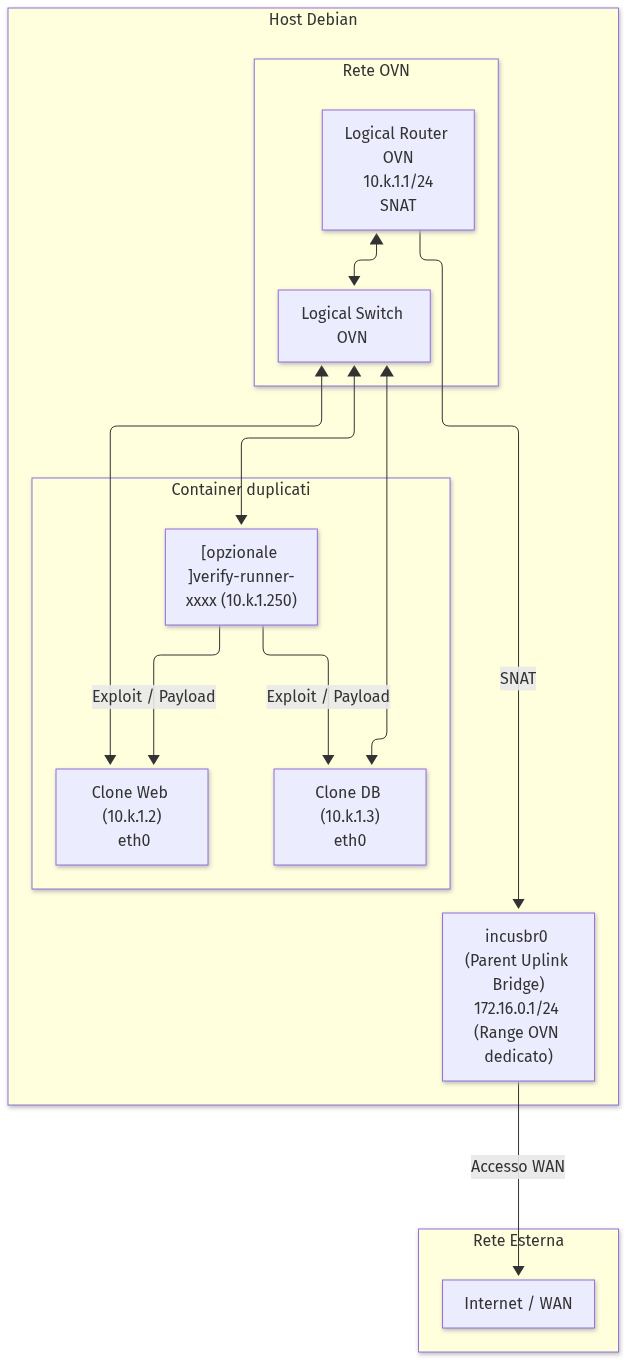
\includegraphics[width=0.92\linewidth,height=0.7\textheight,keepaspectratio]{src/images/mermaid_312_rete_verify_k_d80ab1c21b.png}
  \caption{312 Rete Verify K}
  \label{fig:mermaid_312_rete_verify_k_d80ab1c21b}
\end{figure}

